\documentclass[a4paper]{article}

%--------------------------------------------------------------------------
\usepackage[a4paper, total={6in, 9in}]{geometry}
\usepackage{amsmath}
\usepackage{booktabs}
\usepackage{caption}
\usepackage{graphicx}
\usepackage{float}
\usepackage{inconsolata}
\usepackage{listings}
\usepackage{siunitx}
\usepackage[most]{tcolorbox}
\usepackage{etoolbox}

\makeatletter
\patchcmd{\l@section}
{\hfil}
{\leaders\hbox{\normalfont$\m@th\mkern \@dotsep mu\hbox{.}\mkern \@dotsep mu$}\hfill}
{}{}
\makeatother

%--------------------------------------------------------------------------
\graphicspath{{./fig/}}

%--------------------------------------------------------------------------

\newtcblisting[auto counter]{sexylisting}[2][]{sharp corners, 
    fonttitle=\bfseries, colframe=gray, listing only, 
    listing options={basicstyle=\ttfamily,language=Python}, 
    title=Listing \thetcbcounter: #2, #1}

%--------------------------------------------------------------------------
\begin{document}
\title{HIT332: Embedded and Mobile Systems\\ Practical 1 Notes}
\author{Shane Reynolds}
\maketitle

\tableofcontents

%--------------------------------------------------------------------------
\section{Introduction \& Background}
The intention behind this brief set of notes is to provide guidance on how well the practicals and projects for HIT332: Embedded and Mobile Systems achieve their intended outcomes. There are 5 practicals in total, and 3 projects. This set of notes will cover Practical 1. The practicals (and projects) make use of a development board created by Damien Hill and Ben Saunders of Charles Darwin University. The main component of the board is the Atmel ATmega1281 16au 16MHz, 8-bit microcontroller. The development board can be seen in Figure 1.

\begin{figure}[h]
	\centering
	\frame{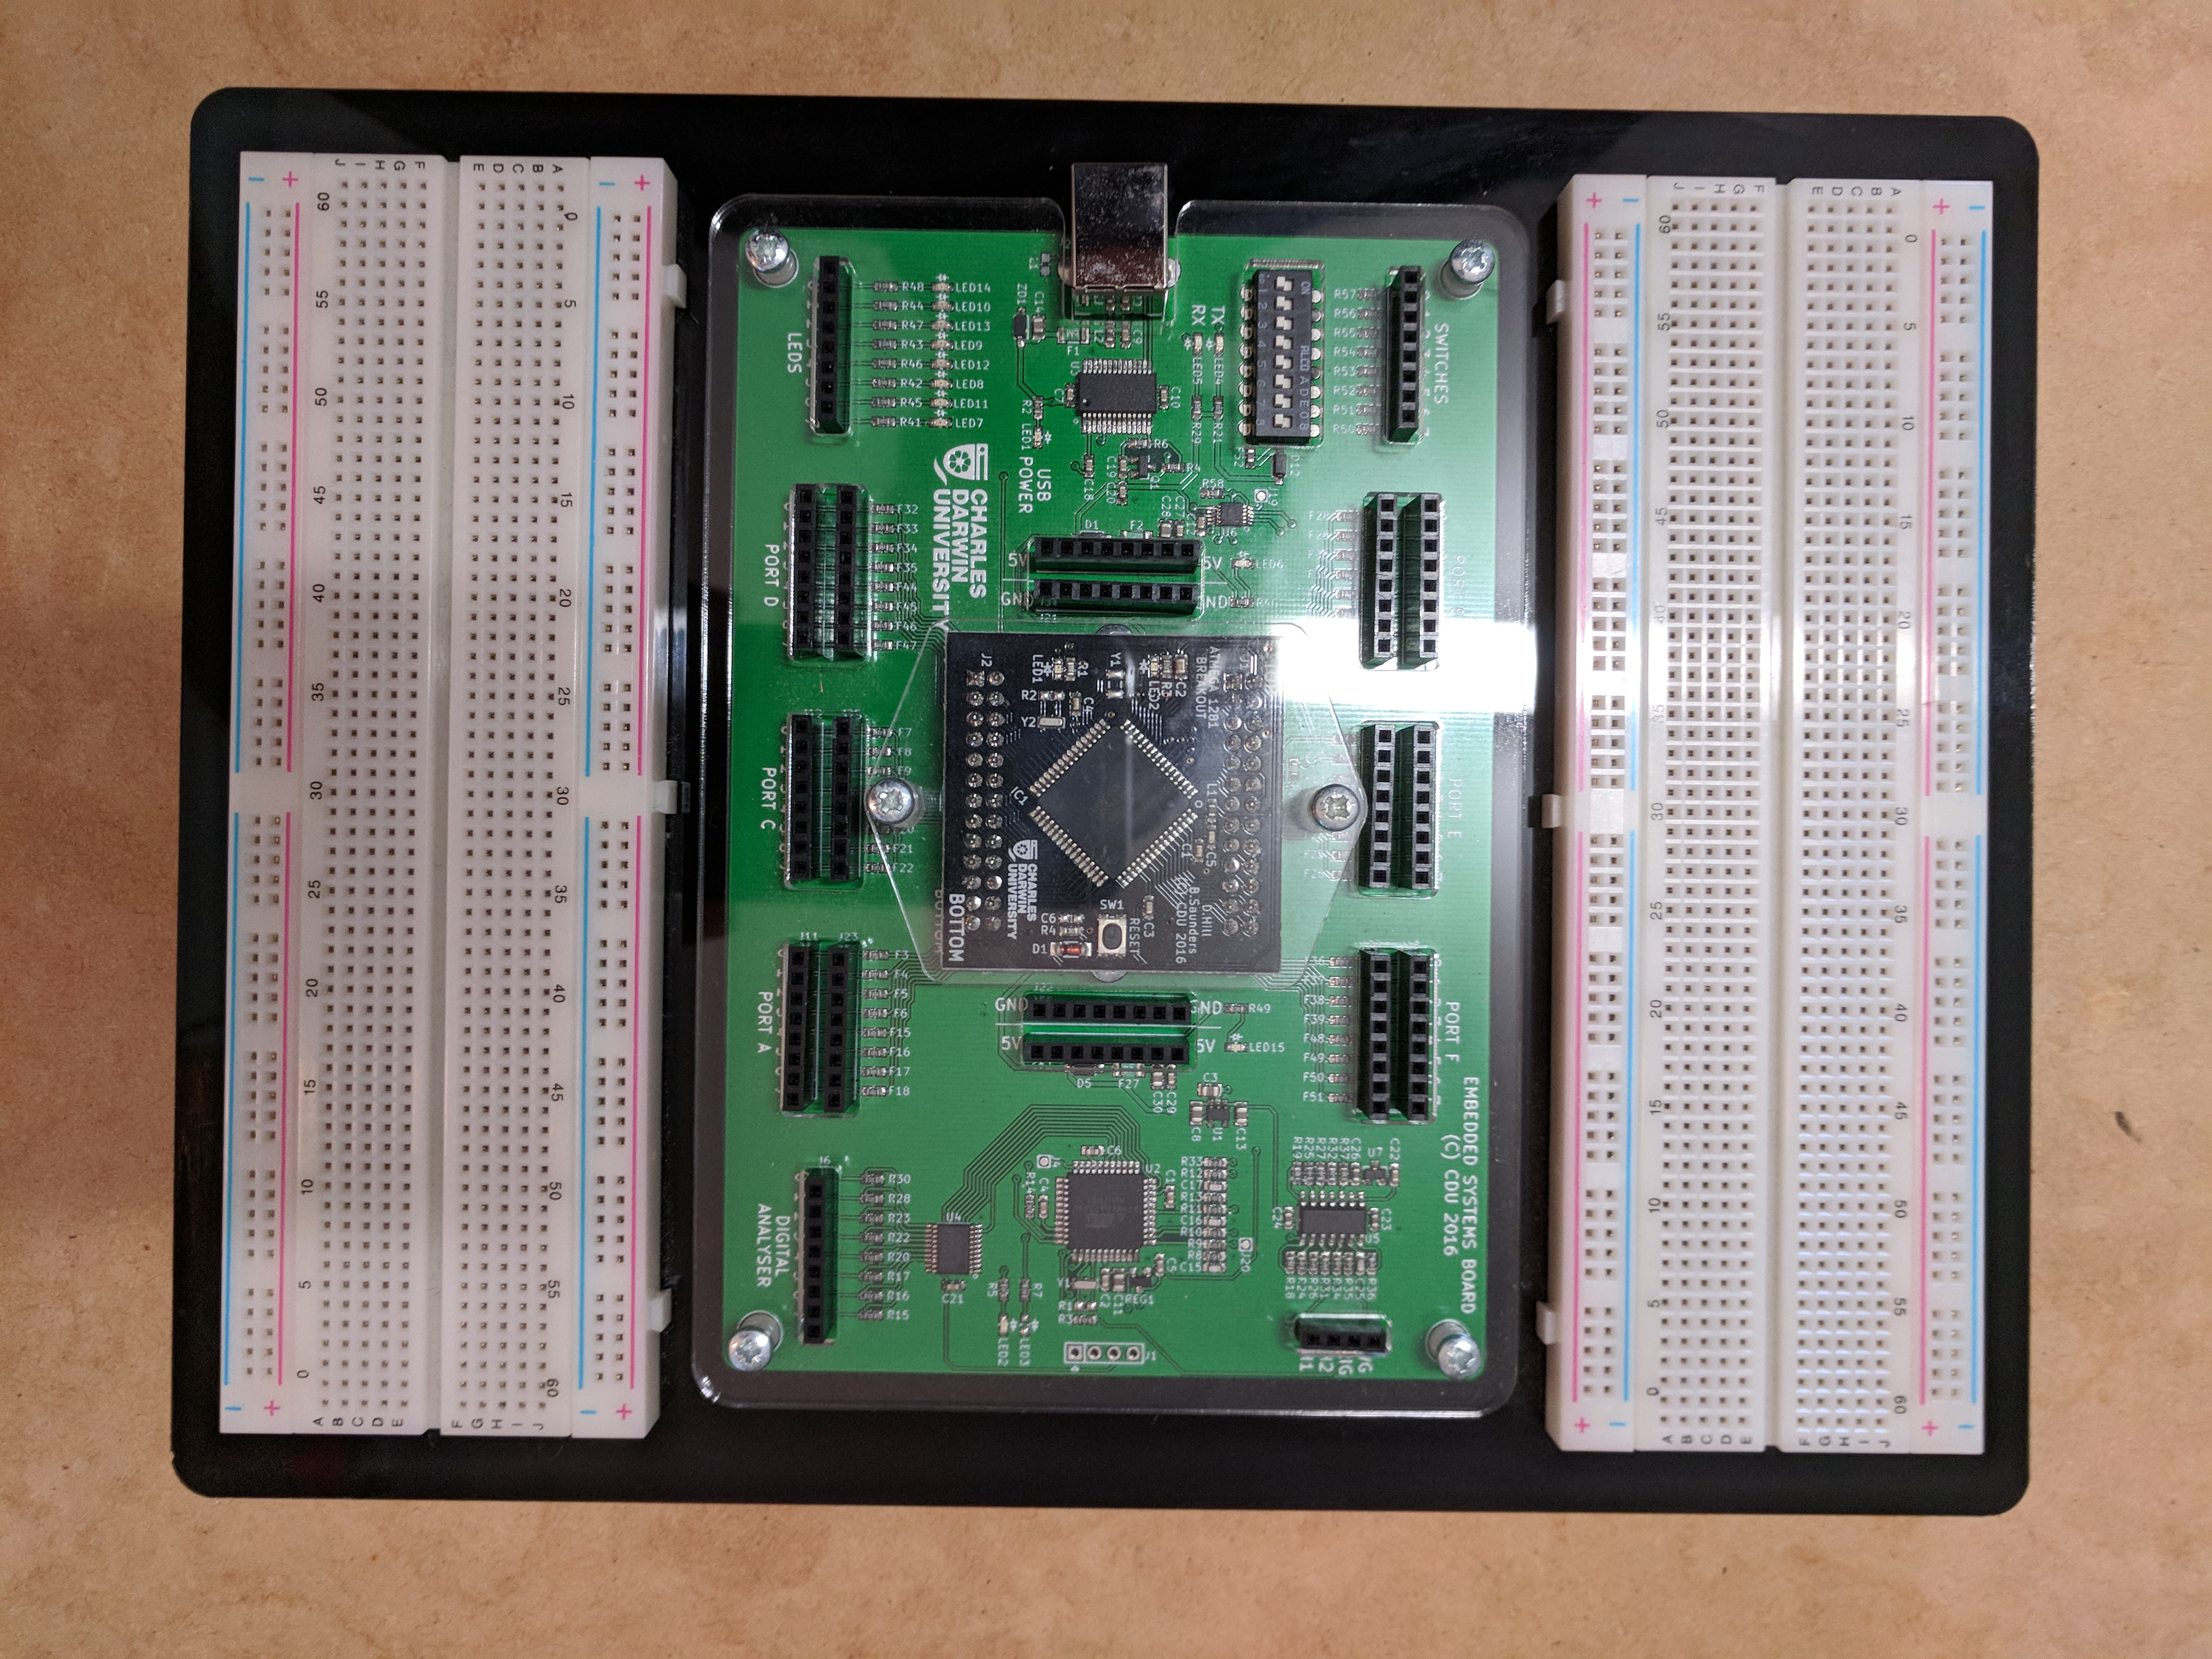
\includegraphics[scale=0.05]{fig1}}
	\caption{The development board which is used in practicals and projects for HIT332: Embedded and Mobile Systems}
\end{figure}

It must be highlighted that these notes have been developed using the board outside of its intended ecosystem. The board is made to be used on CDU's Casuarina Campus in one of the Engineering computer labs. These labs have the appropriate software installed in the correct file paths. These notes have been written using software installed on a personal machine which CDU does not control. Furthermore, the components (other than the development board) used to complete the exercises were sourced independently from a local electronics supplier, independently of CDU. The notes will be highlighted where there has been a significant departure from the intended experience.

\newpage

\section{CDU Embedded System Toolbox}
The CDU Embedded System Toolbox loaded without any problems. The development board was not connected, an error message displayed notifying the user that the board was not connected, and then the interface was displayed with the appropriate buttons were greyed out, as shown in Figure 2.

\begin{figure}[h]
	\centering
	\frame{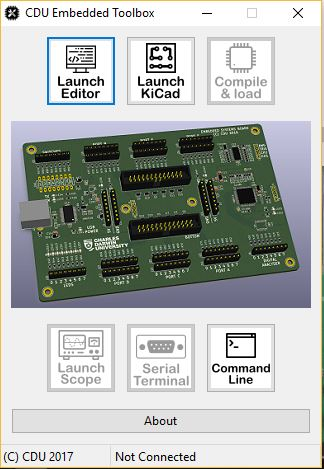
\includegraphics[scale=0.5]{fig2}}
	\caption{The CDU Embedded Toolbox, loaded when the development board is disconnected.}
\end{figure}

\section{KiCad}
KiCAD was installed on the local system being used, however, since it was not installed in the required file path, the CDU Embedded Toolbox did not load. This was expected since the practical is not being done in the required ecosystem. KiCAD worked as expected, and the instructions provided by the practical were fit for purpose. The output from the KiCAD exercise can be seen in Figure 3.

\begin{figure}[h]
	\centering
	\frame{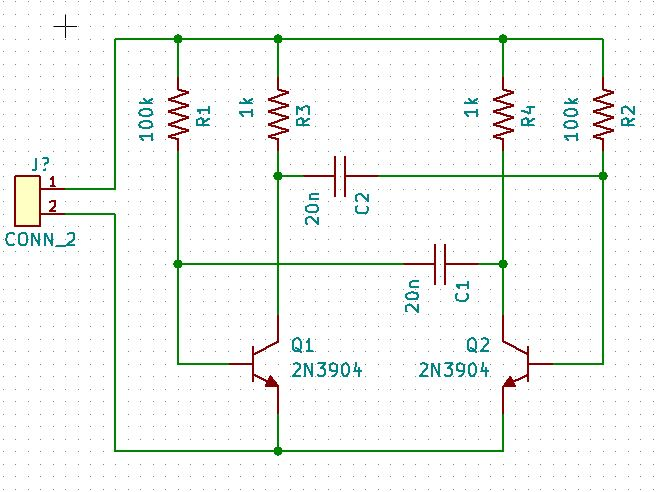
\includegraphics[scale=0.5]{fig3}}
	\caption{The completed exercise using KiCAD and the instructions provided in the practical.}
\end{figure}

\end{document}